\documentclass[10pt]{article}
\setlength{\oddsidemargin}{0in}
\setlength{\evensidemargin}{0in}
\setlength{\textwidth}{7in}
\setlength{\parindent}{0in}
\setlength{\parskip}{\baselineskip}

\usepackage{amsmath,amsfonts,amssymb,bm,graphics,pgfplots,framed,dsfont,mathtools}
\usepackage[scale=0.75,top=1cm,bottom=3cm]{geometry}

\DeclarePairedDelimiter\floor{\lfloor}{\rfloor}

\begin{document}

\textbf{Minh Anh Nguyen }\\
\textbf{Discrete Math\hfill Assignment-10}

\hrulefill

Section 4.1:

\begin{enumerate}
  \item Professor N. Timmy Date has 30 students in his Calculus class and 24 students in his Discrete Mathematics class.
        \begin{enumerate}
          \item Assuming that there are no students who take both classes, how many students does Professor Date have?\\
          Professor Date has a total of 24 + 30 = 54 students.

          \item Assuming that there are eight students who take both classes, how many students does Professor Date have?\\
          Professor Date has a total of 24 + 30 - 8 = 46 students.

        \end{enumerate}

  \item A restaurant offers two different kinds of soup and five different kinds of salad.
        \begin{enumerate}
          \item If you are having either soup or salad, how many choices do you have?\\
          I have 2 + 5 = 7 choices.
          \item If you are having both soup and salad, how many choices do you have?\\
          I have a total of $2 \times 5 = 10$ choices.
        \end{enumerate}

  \item There are 18 major sea islands in the Queen Elizabeth Islands of Canada. There are 15 m\\
        \begin{enumerate}
        \item If you are planning a trip to visit one of these islands, followed by one of these lakes, how many different trips could you make?\\
        I could make a total of 15 x 18 = 270 different trips to make.
        \item If you plan to visit either one of these lakes or one of these islands, how many different visits could you make?\\
        I could make a total of 15 + 18 = 33 different trips to make.
        \end{enumerate}

  \item Bill has three one-piece jumpsuits, five pairs of work pants, and eight work shirts. He wears either a jumpsuit or pants and a shirt to work. How many different possible outfits does he have?\\
  He has $3 \times 5 + 8 = 23$ outfits.

  \item A new car is offered with 10 different optional packages. The dealer claims that there are "more than 1, 000 different combinations" available. Is this claim justified? Explain.\\
  The total combinations is $2^{10} = 1024.$ Hence, this claim is justified.

  \item Suppose that license plates in a certain municipality come in two forms: two letters (A … Z) followed by three digits (0 … 9) or three letters followed by two digits. How many different license plates are possible?\\
        There are a total of 26 + 10 = 36 letters and digits to choose from. Hence there are total $36^3 = 46656$ different license plates.

  \item License plates in India begin with a code that identifies the state and district where the vehicle is registered, and this code is followed by a four-digit identification number. These identification numbers are given sequentially, starting with 0000, 0001, 0002, etc. Once this sequence reaches 9999, a letter from the set {A, …,Z} is added (in order), and once these run out, additional letters are added, and so on. So the sequence of identification numbers proceeds as follows: 0000, 0001, …, 9999, A0000, A0001, …, A9999, B0000, B0001, …, B9999, …, Z0000, Z0001, …, Z9999, AA0000, AA0001, ….
  \begin{enumerate}
    \item How many identification numbers are there that use two or fewer letters?\\
    There are $10000 + 26 \times 10000 + 26 \times 26 \times 10000 = 7030000$ identification numbers.
    \item If a district registers 10 million cars, how many identification numbers must have three letters?\\
    There are $10,000,000 - 7030000 = 2970000$ identification numbers have 3 letters.
    \item Suppose a district registers 500,000 cars. What percentage of identification numbers have exactly one letter?\\
    The percentage is $\frac{26 \times 10000}{500,000} \times 100 = 52\%$
    \item Suppose a district registers 500,000 cars. What percentage of identification numbers have no letters?\\
    The percentage is $\frac{10000}{500,000} \times 100 = 2\%$
    \item Suppose you see a plate in Bangalore, India, with the identification number CR7812. How many vehicles were registered in this district before the vehicle with this plate?\\
    The number of vehicles registered before this identification numbers is $7812 + 10000 \times 26 + 10000 \times 26 \times 3 + 17 \times 10000 -1 = 1217811$
  \end{enumerate}

  \item License plates in China begin with a Chinese character designating the province, followed by a letter from the set {A, …, Z}, followed by a five-character alphanumeric string (using symbols from the set {A, …, Z, 0, 1,…9}. What is the maximum number of plates of this type for a given Chinese province?\\
  The maximum number of plates is $26 + (26+10)^5 = 60466202$.

  \item The protein-coding strand of the average human gene consists of 1,350 nucleotides. Assuming that each nucleotide can take any of four values (A, T, C, or G), how many different genes with exactly 1,350 nucleotides are possible?\\
  There are $4^{1350}$ different genes possible.

  \item Refer to the previous problem. Assuming that gene strands can have between 1,200 and 1,500 nucleotides, write an expression for the number of possible genes. (Don’t bother trying to evaluate this expression!)
  \[\Sigma_{n=1200}^{1500} 4^n\]

  \item How many numbers between 1 and 999 (inclusive) are divisible by either 2 or 5?
  There are $\floor[\Bigg]{\frac{999}{2}} + \floor[\Bigg]{\frac{999}{5}} = 499 + 199 = 698$

\end{enumerate}

Section 4.2:

\begin{enumerate}
  \item Arturo can have pizza for dinner on any three of the next seven days. How many different ways can he select the days on which to have pizza?\\
  There are $C(7,3) = 35$ different ways.
  \item There are 13 different pizza toppings, and Arturo must rank his top 5 in order. How many different possible rankings are there?\\
  There are $P(13,5) = 154440$ rankings.
  \item A committee of three is chosen from a group of 20 people. How many different committees are possible, if
  \begin{enumerate}
    \item the committee consists of a president, vice president, and treasurer?
    There are $P(20,3) = 6840$ different committees possible.
    \item there is no distinction among the three members of the committee?
    There are $C(20,3) = 1140$ different committees possible.
  \end{enumerate}

  \item Hugo and Viviana work in an office with eight other coworkers. Out of these 10 workers, their boss needs to choose a group of four to work together on a project.
  \begin{enumerate}
    \item How many different working groups of four can the boss choose?\\
    The boss can choose $C(10,4) = 210$ working groups.
    \item Suppose Hugo and Viviana absolutely refuse, under any circumstances, to work together. Under this restriction, how many different working groups of four can be formed?\\
    There are $C(9,4) + C(9,4) + C(8,4) = 322$ possible groups.
  \end{enumerate}

  \item Ruth has the following set of refrigerator magnets: \{A, B, C, D, E, F, G\}.
  \begin{enumerate}
    \item How many different three-letter strings can she form with these magnets?\\
    There are $C(7,3) = 35$ different three-letter strings can be formed.
    \item How many different three-letter strings can she form if the middle letter must be a vowel?\\
    There are $C(5,2) \times C(2,1) = 20$ different three-letter strings can be formed.
  \end{enumerate}

  \item Refer to Example 4.22. Use the selection principle to count the number of different possible win or loss scenarios when two teams play a best-of-five match …
  \begin{enumerate}
    \item using the method of Solution $1$.
    \[\text{Total scenarios} = 2 + 2 \times C(3,1) + 2 \times C(4,2) = 20\]
    \item using the method of Solution $2$.
    \[\text{Total scenarios} = C(5,3) + C(5,3) = 20\]
  \end{enumerate}

  \item Form a seven-letter word by mixing up the letters in the word COMBINE.
  \begin{enumerate}
    \item How many ways can you do this?
    There are $P(7,7) = 5040$ ways.
    \item How many ways can you do this if all the vowels have to be at the beginning?
    There are $P(3,3) x P(4,4) = 144$ ways.  
    \item How many ways can you do this if no vowel is isolated between two consonants?
    There are $P(5,5) \times P(3,3) = 720$ ways.  
  \end{enumerate}

  \item How many different strings can be formed by rearranging the letters in the word ABABA?\\
  There are $C(5,3) = 10$ different strings can be formed.  
  
  \item Lipid Fried Chicken offers a jumbo special with a choice of three side dishes from eight different side dishes on the menu. Assuming you must choose three different side dishes, how many different possibilities are there for your side dish selection?\\
  There are $C(8,3) = 56$ different possibilities.

  \item Possible grades for a class are A, B, C, D, and F. 
  \begin{enumerate}
    \item How many ways are there to assign grades to a class of seven students?\\
    There are $5^7 = 78125$ ways.
    \item How many ways are there to assign grades to a class of seven students if nobody receives an F and exactly one person receives an A?\\
    There are $3^6 \times 7 = 5103$ ways.
  \end{enumerate}

  \item The school board consists of three men and four women.
  \begin{enumerate}
    \item When they hold a meeting, they sit in a row. How many different seating arrangements are there?\\
    There are $P(7,7) = 5040$ seating arrangements.
    \item How many different ways can the row be arranged if no two women sit next to each other?\\
    There are $P(3,3) \times P(4,4) = 144$ seating arrangements.
    \item How many ways are there to select a subcommittee of four board members?\\
    There are $C(7,4) = 35$ ways to select a subcommittee of four board members.
    \item How many ways are there to select a subcommittee of four board members if the subcommittee must contain at least two women?\\
    There are $C(4,2) \times C(3,2) + C(4,3) \times C(3,1) + C(4,4) = 31$ ways to select a subcommittee of four board members.
  \end{enumerate}

\setcounter{enumi}{15}

  \item Using the nouns N = {dog, man, mouse, bird} and the verbs V = {bites, eats, kicks}, how many “sentences” of the form
  \[\text{Noun      Verb      Noun}\]
  are there, with the restriction that every word in the sentence has a different length? (For example, “dog eats mouse” is such a sentence, but “man bites dog” is not, because it contains two words of length three.) Use a decision tree to arrive at your answer.\\
  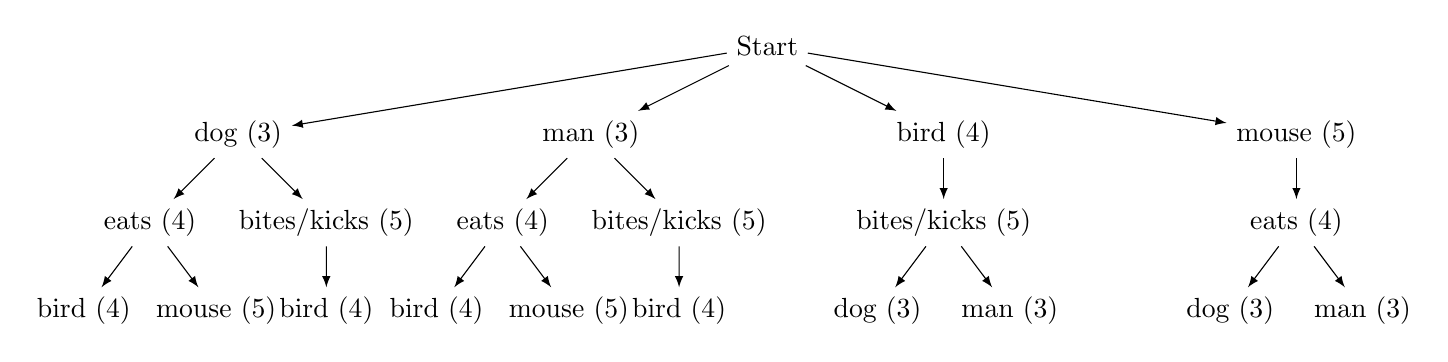
\begin{tikzpicture}[
    scale=0.56,
    level distance=2cm,
    level 1/.style={sibling distance=8cm},
    level 2/.style={sibling distance=4cm},
    level 3/.style={sibling distance=3cm},
    edge from parent/.style={draw, -latex}
  ]
  
  % Root node
  \node {Start}
    % Level 1: First Noun
    child {node {dog (3)}
      % Level 2: Verb choices
      child {node {eats (4)}
        % Level 3: Second Noun choices
        child {node {bird (4)}}
        child {node {mouse (5)}}
      }
      child {node {bites/kicks (5)}
        child {node {bird (4)}}
      }
    }
    child {node {man (3)}
      child {node {eats (4)}
        child {node {bird (4)}}
        child {node {mouse (5)}}
      }
      child {node {bites/kicks (5)}
        child {node {bird (4)}}
      }
    }
    child {node {bird (4)}
      child {node {bites/kicks (5)}
        child {node {dog (3)}}
        child {node {man (3)}}
      }
    }
    child {node {mouse (5)}
      child {node {eats (4)}
        child {node {dog (3)}}
        child {node {man (3)}}
      }
    };
  
  \end{tikzpicture}
  There are 14 valid sentences.

\setcounter{enumi}{19}
  \item Find an alternate solution to Exercise 19. (Count the number of strings that contain 000 or 111 and subtract from the total number of four-digit binary strings.)\\
  There are $2^4 - 4 = 12$ strings.
\end{enumerate}

\end{document}